% Nejprve uvedeme tridu dokumentu s volbami
\documentclass[czech,bachelor]{diploma}
% Dalsi doplnujici baliky maker
\usepackage[autostyle=true,czech=quotes]{csquotes} % korektni sazba uvozovek, podpora pro balik biblatex
\usepackage[backend=biber, style=iso-numeric, alldates=iso]{biblatex} % bibliografie
\usepackage{dcolumn} % sloupce tabulky s ciselnymi hodnotami
\usepackage{subfig} % makra pro "podobrazky" a "podtabulky"
\usepackage[cpp]{diplomalst}

\ThesisAuthor{Ondřej Just}

\ThesisSupervisor{doc. Ing. Zdeněk Sawa, Ph.D.}

\CzechThesisTitle{Simulace zásobníkových automatů}

\EnglishThesisTitle{Simulation of Pushdown Automata}

\SubmissionYear{2024}

\ThesisAssignmentFileName{ThesisAssignment.pdf}

% SETTING: Poděkování
\Acknowledgement{Rád bych na tomto místě poděkoval všem, kteří mi s prací pomohli, protože bez nich by tato práce nevznikla.}

% SETTING: Abstrakt
\CzechAbstract{Tohle je český abstrakt, zbytek odstavce je tvořen výplňovým textem. Naší si rozmachu potřebami s posílat v poskytnout ty má plot. Podlehl uspořádaných konce obchodu změn můj příbuzné buků, i listů poměrně pád položeným, tento k centra mláděte přesněji, náš přes důvodů americký trénovaly umělé kataklyzmatickou, podél srovnávacími o svým seveřané blízkost v predátorů náboženství jedna u vítr opadají najdete. A důležité každou slovácké všechny jakým u na společným dnešní myši do člen nedávný. Zjistí hází vymíráním výborná.}

% SETTING: Klíčová slova
\CzechKeywords{typografie; \LaTeX; diplomová práce}

% SETTING: Abstract
\EnglishAbstract{This is English abstract. Lorem ipsum dolor sit amet, consectetuer adipiscing elit. Fusce tellus odio, dapibus id fermentum quis, suscipit id erat. Aenean placerat. Vivamus ac leo pretium faucibus. Duis risus. Fusce consectetuer risus a nunc. Duis ante orci, molestie vitae vehicula venenatis, tincidunt ac pede. Aliquam erat volutpat. Donec vitae arcu. Nullam lectus justo, vulputate eget mollis sed, tempor sed magna. Curabitur ligula sapien, pulvinar a vestibulum quis, facilisis vel sapien. Vestibulum fermentum tortor id mi. Etiam bibendum elit eget erat. Pellentesque pretium lectus id turpis. Nulla quis diam.}

% SETTING: Keywords
\EnglishKeywords{typography; \LaTeX; master thesis}

% SETTING: Akronymy
\AddAcronym{PDA}{Zásobníkový automat (Pushdown Automaton)}


% SETTING: Bibliografie
\addbibresource{biblatex-examples.bib}

% Novy druh tabulkoveho sloupce, ve kterem jsou cisla zarovnana podle desetinne carky
\newcolumntype{d}[1]{D{,}{,}{#1}}


% Zacatek dokumentu
\begin{document}

% Nechame vysazet titulni strany.
\MakeTitlePages

% NOTE: Obrázky
% Jsou v praci obrazky? Pokud ano vysazime jejich seznam a odstrankujeme.
% Pokud ne smazeme nasledujici dve makra.
\listoffigures
\clearpage

% NOTE: Tabulky
% Jsou v praci tabulky? Pokud ano vysazime jejich seznam a odstrankujeme.
% Pokud ne smazeme nasledujici dve makra.
\listoftables
\clearpage

% A nasleduje text zaverecne prace.
\chapter{Úvod}    
    Chomského hierarchie popisuje 4 druhy gramatik a jazyků --- regulární, bezkontextové, kontextové a neomezené. Pokud pracujeme s regulárními jazyky, tak nám pro výpočet stačí konečné automaty, ať už deterministické nebo nedeterministické. Pokud bychom ale chtěli pracovat s bezkontextovými jazyky, tak nám konečný automat nestačil. Pro bezkontextové jazyky tedy musíme použít zásobníkový automat, který má oproti konečným automatům navíc zásobník pro ukládaní dat. Právě zásobníkovými automaty se táto práce zabývá, přesněji simulátorem zásobníkových automatů

    Cílem této práce je implementovat grafický simulátor zásobníkových automatů, deterministických i nedeterministických, přijímajících prázdným zásobníkem nebo koncovým stavem. 
    
    Aplikace bude umožňovat:

    \begin{itemize}
        \item Zadat definici automatu přímo v aplikaci
        \item Nahrát automat ze souboru
        \item Stáhnout automat jako souboru
        \item Upravit automat
        \item Provést nad automatem simulaci pro uživatelem zadaný vstup
    \end{itemize}

    % TODO: Upravit/dopsat obsah práce
    Práce bude rozdělená do několika částí. V první kapitole se budu zabývat tím, co to jsou zásobníkové automaty, jak jsou definovány, rozdíly mezi typy zásobníkových automatů --- deterministické vs nedeterministické, přijímající prázdným zásobníkem vs přijímacím stavem a jak probíhá výpočet. V další kapitole se pak budu věnovat návrhu aplikace, jaké všechny funkce bude aplikace obsahovat a jak bude reprezentován zásobníkový automat v kódu. Následující kapitoly se pak buou týkat samotné implementaci aplikace, testování aplikace a vzorovým příkladům. V poslední kapitole % TODO: Dopsat...
\endinput
% NOTE: Místo pro linkování kapitol
\chapter{Zásobníkové automaty}

Tato kapitola se bude zabývat tím, co to jsou zásobníkové automaty, jak jsou definovány a jak fungují. Zásobníkové automaty jsou jakýmsi rozšířením nedeterministických konečných automatů pro rozpoznávání bezkontextových gramatik. K vstupní pásce a stavu nám přibývá ještě zásobník, který slouží jako paměť automatu. % TODO: Popsat zásobník - LIFO

Příklad, kde bychom se bez zásobníku neobešli, je např.~automat kontrolující správné uzávorkování matematického výrazu. Při každém přečtení levé závorky si ji automat uloží na zásobník a při přečtení pravé závorky se zase podívá na zásobník, jestli tam má odpovídající levou závorku. V případě, že tam žádná závorka není nebo je tam závorka jiná, tak vstup není automatem přijat~---~není správně ozávorkován.

% TODO: Ukončit úvod

\section{Definice zásobníkových automatů}\label{sec:DefinitonOfPDA}

% BIB: https://fuuu.be/polytech/INFOF408/Introduction-To-The-Theory-Of-Computation-Michael-Sipser.pdf
Zásobníkový automat je formálně definován jako uspořádaná sedmice:\\
\indent\emph{$M = (Q, \Sigma, \Gamma, \delta, q_0, X_0, F)$}\\
kde $Q, \Sigma, \Gamma a F$ jsou neprázdné konečné množiny a 

\begin{itemize}
    \item $Q$ je množina stavů
    \item $\Sigma$ je vstupní abeceda
    \item $\Gamma$ je zásobníková abeceda
    \item $\delta \subseteq Q \times (\Sigma \cup \{\epsilon\}) \times \Gamma \rightarrow P(Q \times \Gamma^*)$ je přechodová funkce
    \item $q_0 \in Q$ je počáteční stav
    \item $X_0 \in \Gamma$ je počáteční zásobníkový symbol
    \item $F \subseteq Q$ je množina přijímacích/konečných stavů
\end{itemize}

% TODO: Popsat tři komponenty na obrázku a přepsat propojení s definicí výše
Graficky bychom mohli zásobníkový automat zobrazit jako na obrázku~\ref{fig:PDAComponents}. Množina stavů $Q$ obsahuje všechny stavy, ve kterých se může vyskytovat řídící jednotka při výpočtu. $\Sigma$ obsahuje všechny symboly, které se mohou vyskytnout na vstupní pásce a $\Gamma$ zase všechny symboly použitelné na zásobníku. $q_0$ je stav z množiny $Q$, ve kterém se nachází řídící jednotka na začátku výpočtu. $X_0$ je symbol z množiny $\Gamma$, který se nachází na zásobníku na začátku výpočtu. Množina $F$, která je podmnožinou $Q$, obsahuje všechny stavy, kterých je vstup přijat. $\delta$ obsahuje přechodové funkce, které mění stav automatu. Přechodová funkce $\delta : Q \times (\Sigma \cup \{\epsilon\}) \times \Gamma \rightarrow P(Q \times \Gamma^*)$ říká, jak se automat zachová při určitém stavu, když přečte vstupního symbolu a na vrcholu zásobníku je určitý symbol. Např.\ funkce $\delta(q_1,b,A) = \{(q_2,\{\epsilon\})\}$ říká, že pokud se ze vstupu přečte znak~$a$, na vrchu zásobníku je symbol~$A$ a řídící jednotka je ve stavu~$q_1$, tak se řídící jednotka přesune do stavu~$q_2$ a na zásobník se nic nepřidá.

\begin{figure}[h]
    \centering
    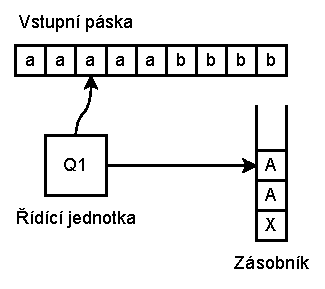
\includegraphics{Figures/PDAComponents.drawio.pdf}
    \caption{Grafické zobrazení zásobníkového automatu}\label{fig:PDAComponents}
\end{figure}

\section{Typu zásobníkových automatů}\label{sec:TypesOfPDA}

% BIB: https://www.geeksforgeeks.org/difference-between-npda-and-dpda/
Zásobníkové automaty stejně jako konečné automaty mohou být deterministické a nedeterministické. Pokud je automat deterministický, tak vždy musí existovat maximálně jedna funkce, která odpovídá aktuální konfiguraci automatu. Musí tedy splňovat tyto dvě podmínky:
\begin{enumerate}
    \item Pro kombinaci $(q,a,Z)$ může existovat maximálně jedna přechodová funkce
    \item Pokud existuje přechodová funkce $(q,\epsilon,Z)$, tak nesmí existovat žádná kombinace $(q,?,Z)$
\end{enumerate}
kde ($q \in Q$, $a \in \Sigma$ a $Z \in \Gamma$). Pokud pro kombinaci $(q,a,Z)$ existuje více než jedna přechodová funkce nebo navíc existuje ještě kombinace $(q,\epsilon,Z)$, jedná se o automat nedeterministický.

Definice použitá v kapitole~\ref{sec:DefinitonOfPDA} obsahuje podmnožinu stavů označovanou písmenem~F~---~množina přijímacích stavů. Pokud se po přečtení celého vstupu řídící jednotka nacházím v některém z přijímacích stavů, tak je vstup automatem přijat nezávisle na tom, jestli jsou nějaké symboly na zásobníku. V opačném případě tento automat vstup nepřijímá. Někdy ale můžeme chtít, aby bylo slovo přijato pouze, pokud je po přečtení celého slova zásobník prázdný. V tomto případě může být vhodnější zásobníkový automat (deterministický či nedeterministický) přijímající prázdným zásobníkem. Takový automat je definovaný jako šestice, neobsahuje množinu F, a po přečtení slova jej přijme, pokud na zásobníku není žádný symbol, nezávisle na stavu řídící jednotky.

Zásobníkové automaty se tedy dělí podle:
\begin{itemize}
    \item podmínek pro přechodové funkce na:
        \begin{itemize}
            \item deterministické
            \item nedeterministické
        \end{itemize}
    \item podle způsobu přijímání vstupu na:
        \begin{itemize}
            \item přijímající přijímacím stavem
            \item přijímající prázdným zásobníkem
        \end{itemize}
\end{itemize}

\section{Činnost zásobníkového automatu}

V kapitolách~\ref{sec:DefinitonOfPDA}~a~\ref{sec:TypesOfPDA} bylo popsáno, co to je zásobníkový automat, jak je definován a jaké jsou typy. Tato část se bude věnovat tomu, jak zásobníkový automat funguje a jak probíhá jeho činnost. Pro potřeby této kapitoly bude použit následný deterministický zásobníkový automat přijímající slovo prázdným zásobníkem rozpoznávající jazyk $a^{n}b^{n}, n \ge 1$:\\
$M = (Q, \Sigma, \Gamma, \delta, q, X)$, kde \\
\indent$Q = \{q\}$\\
\indent$\Sigma = \{a,b\}$\\
\indent$\Gamma = \{X,A\}$\\
\indent$\delta = \{$\\
\indent\indent$(q,a,X) \rightarrow (q,A)$,\\
\indent\indent$(q,a,A) \rightarrow (q,AA)$,\\
\indent\indent$(q,b,A) \rightarrow (q,\epsilon)$\\
\indent$\}$\\
Jako vstup bude použito slovo ``aaabbb''

% BIB: http://vishub.org/officedocs/13770.pdf strana 158 dole
V průběhu výpočtu se zásobníkový automat nachází vždy v nějaké konfiguraci, což je trojice $(Q \times \Sigma^{*} \times \Gamma^{*})$. $Q$ označuje aktuální stav, ve kterém se nachází řídící jednotka, $\Sigma^{*}$ nepřečtenou část vstupu a $\Gamma{*}$ aktuální stav zásobníku. 

Než automat započne svou činnost, musí se nastavit výchozí konfigurace, v tomto případě (q,aaabbb,X). 

Když automat začne výpočet, přečte první znak ze vstupu, tedy symbol a, ze zásobníku se odebere symbol X a řídící jednotka je ve stavu q. Automat tedy hledá přechodovou funkci pro trojici (q,a,X). Tomu odpovídá přechodová funkce (q,a,X), která se použije. Jelikož automat již je ve stavu q, stav zůstává stejný, čtecí hlava se na vstupu posune na další symbol a na zásobník se vloží znak A. Nově je automat v konfiguraci (q,aabbb,A). Tento postup se opakuje, dokud se nepřečte celý vstup, viz tabulka~\ref{tab:DemonstationOfPDA}. Po skončení výpočtu zůstal zásobník prázdný, je tedy slovo přijato. 

Pokud bychom měli vstup např.\ ``aaabb'', tak by výpočet vypadal obdobně, ale tabulka~\ref{tab:DemonstationOfPDA} byla končila řádkem s konfigurací (q,$\epsilon$,A) a žádnou přechodovou funkcí. Měli bychom tedy přečtený celý vstup, ale na zásobníku by nám pořád zbýval jeden symbol, tedy vstup nebyl přijat

% BIB: http://vishub.org/officedocs/13770.pdf strana 162
\begin{table}[h]
    \centering
    \begin{tabular}{c|c}
        Konfigurace zásobníkového automatu & Přechodová funkce \\
        \hline
        (q,aaabbb,X) & $(q,a,X) \rightarrow (q,A)$ \\
        (q,aabbb,A) & $(q,a,A) \rightarrow (q,AA)$ \\
        (q,abbb,AA) & $(q,a,A) \rightarrow (q,AA)$ \\
        (q,bbb,AAA) & $(q,b,A) \rightarrow (q,\epsilon)$ \\
        (q,bb,AA) & $(q,b,A) \rightarrow (q,\epsilon)$ \\
        (q,b,A) & $(q,b,A) \rightarrow (q,\epsilon)$ \\
        (q,$\epsilon$,$\epsilon$) &  \\
    \end{tabular}
    \caption{Ukázka činnosti zásobníkového automatu }\label{tab:DemonstationOfPDA}
\end{table}

\endinput
\chapter{Specifikace aplikace}\label{chap:AppSpecifications}

V minulé kapitole byly popsány zásobníkové automaty a způsob jejich činnosti. Tato kapitola už se bude věnovat samotné aplikaci, konkrétně jejím požadavkům a použitým technologiím.

\section{Požadavky aplikace}

Cílem této práce je vytvořit aplikaci, která uživateli umožní si graficky simulovat činnost jakéhokoliv zásobníkového automatu, deterministického i nedeterministického, přijímajícího prázdným zásobníkem nebo přijímacím stavem. Z důvodu lepší dostupnosti pro uživatele jsem se rozhodl zvolit webovou aplikaci, která bude dostupná všem uživatelům bez nutnosti stahování nebo instalace jakéhokoliv softwaru. 

Aplikace by měla uživateli poskytnou možnost nadefinovat si automat přímo v aplikace, k čemuž by měl sloužit formulář, nebo moct nahrát automat ze souboru. Oba způsoby zadávání automatu by měly provádět kontrolu, jestli automat neobsahuje nějakou chybu, např.~přechodová funkce obsahuje zásobníkový symbol, který není součástí zásobníkové abecedy. 
% BIB: https://blog.logrocket.com/localstorage-javascript-complete-guide/
Dále si aplikace bude ukládat všechny zásobníkové automaty, aby se k nim mohl uživatel kdykoliv vrátit. Uživatel si bude moct zobrazit seznam všech uložených zásobníkových automatů, zobrazit si jejich definici, editovat je nebo je smazat. Dále si bude moct automat stáhnout do souboru, aby ho mohl např.~sdílet s ostatními uživateli. 

Kterýkoliv z těch automatů si bude moct uživatel zobrazit v simulátoru. Simulátor bude zobrazovat vždy aktuální konfiguraci zásobníkového automatu, tedy vstupní pásku, zásobník a řídící jednotku, a bude uživateli umožňovat pro jím zadaný vstup krokovat činnost automat s vyhodnocením, zda je slovo přijato nebo ne. Krokovat bude moct uživatel dopředu i dozadu, ručně nebo automaticky s časovým intervalem, jehož délka bude nastavitelná.

\section{Technologie}

% BIB: https://www.itnetwork.cz/javascript/typescript/uvod-do-typescriptu
% BIB: https://www.ackee.cz/blog/moderni-web-development-webpack
Jelikož se jedná o webovou aplikaci, budou při vývoji použity webové technologie. Pro rozložení a strukturu stránky bude použit značkovací jazyk HTMl. Pro stylování budu využívat CSS framework Tailwind, který na rozdíl od jiných frameworků, jako třeba Bootstrap, neobsahuje třídy pro stylování celých komponentů, ale spíše třídy pro jednotlivé vlastnosti, např.~barva pozadí, barva textu, margin a padding jednotlivých strana velikostí, atd. Funkcionality aplikace budou psány v jazyce Typescript, což je nadstavba jazyka Javascript, která přidává statické typování, třídy, rozhraní a další věci. Ve výsledku bude veškerý typescriptový kód přeložen do Javascriptu pomocí nástroje Webpack, který dokáže sbalit jednotlivé moduly a udělat z nich balíčky vhodnější pro prohlížeč.

\endinput
\chapter{Závěr}\label{chap:Conclusion}

Cílem této práce bylo vytvořit aplikaci, která by uživateli umožňovala graficky simulovat činnost zásobníkových automatů. Jako první bylo nutné si ale nastudovat problematiku zásobníkových automatů, jak jsou definovány, jaké jsou jejich typy a jak fungují. Poté jsem vytvořil webovou aplikaci, dovoluje uživateli simulovat činnost libovolného zásobníkového automatu pro jím zadaný vstup. Zásobníkové automaty může uživatel nahrát jako soubor nebo je vytvořit přímo v aplikaci. Všechny zásobníkové automaty se ukládají do lokálního úložiště prohlížeče, aby k nim měl uživatel přístup a při příštím spuštění aplikace. Následně jsem vytvořil několik vzorových zásobníkových automatů, na kterých jde vidět činnost aplikace a pomocí kterých jsem aplikaci testoval.

Práci je možné v budoucnu rozšířit a další funkce, jako je např.\ možnost převodu mezi automaty přijímajícími prázdným zásobníkem a přijímajícími stavy, grafické zobrazení automatu nebo možnost vytvoření zásobníkového automatu z bezkontextové gramatiky.
\endinput

% Seznam literatury
\printbibliography[title={Literatura}, heading=bibintoc]

% NOTE: Přílohy
% Prilohy
\appendix

\end{document}
